% This is samplepaper.tex, a sample chapter demonstrating the
% LLNCS macro package for Springer Computer Science proceedings;
% Version 2.20 of 2017/10/04
%
\documentclass[tikz,runningheads,a4paper]{llncs}
%
\usepackage[portuges]{babel}
\usepackage[utf8x]{inputenc}

\usepackage{graphicx}
% Used for displaying a sample figure. If possible, figure files should
% be included in EPS format.
%
% If you use the hyperref package, please uncomment the following line
% to display URLs in blue roman font according to Springer's eBook style:
% \renewcommand\UrlFont{\color{blue}\rmfamily}

%% Useful packages
\usepackage[font=small,labelfont=bf]{caption} % Required for specifying captions to tables and figures

\graphicspath{ {./Images/} }
\usepackage[colorlinks=False]{hyperref} % add links inside PDF files
\usepackage{amsmath}  % Math fonts
\usepackage{amsfonts} %
\usepackage{amssymb}  %
\usepackage{multirow}
\usepackage{float}
\usepackage{cite}
\usepackage{tikz-cd} 

\begin{document}
%
\title{CLAV - ESPECIFICAÇÃO E VERIFICAÇÃO DO MODELO FORMAL}
%
%\titlerunning{Abbreviated paper title}
% If the paper title is too long for the running head, you can set
% an abbreviated paper title here
%
\author{Armando Santos \and
Gonçalo Duarte}

%
\authorrunning{A. et al.}
% First names are abbreviated in the running head.
% If there are more than two authors, 'et al.' is used.
%
\institute{University of Minho, Braga, Portugal}
%
\maketitle              % typeset the header of the contribution
%
\begin{abstract}

CLAV é uma plataforma que está a ser desenvolvida pelo Departamento de Informática da Universidade do Minho em parceria com a Direção Geral do Livro, Arquivos e Bibliotecas (DGLAB), e tem como objetivo a classificação e avaliação de todos os documentos que circulam pelas instituições públicas portuguesas. Neste momento existe um modelo do problema especificado em OWL (\textit{Ontology Web Language}), mas tem sofrido várias alterações no decorrer do último ano e não existiu tempo para estudar o impacto dessas mesmas alterações nas pré-condições e invariantes do modelo. Neste projeto, inserido na Unidade Curricular de Laboratórios em Engenharia Informática (LEI) do MIEI/UM, pretende-se formalizar o modelo de raíz assim como os seus invariantes e garantir a consistência dos mesmos, sendo capaz de detetar erros que, até agora, não tenham sido identificados.

\keywords{Administração Pública \and Métodos Formais \and Engenharia Informática \and Alloy Analyzer \and OWL.}
\end{abstract}
%
%
%
\section{Introdução}

Até agora, em Portugal, não existia nenhum sistema de informação que gerisse a classificação e a avaliação dos documentos gerados no âmbito dos processos que circulam dentro das instituições públicas portuguesas. O CLAV veio mudar isso com a elaboração de um catálogo, que se pretende que venha a ser a referência nacional de todos processos da Administração Pública (AP), tendo sido modelado numa ontologia. Esta ontologia está especificada num modelo formal que representa o conjunto de conceitos referentes aos processos de negócio e aos relacionamentos entre eles. Infelizmente, todos os dados e documentação de apoio estão espalhados, desorganizados e em diferentes formatos, o que os torna extremamente difíceis de manter num domínio tão complexo como o da AP. No entanto, embora já tenham sido feitos esforços para criar um formato neutro, como a Macro-estrutura Funcional (MEF), e vários sistemas de exploração e exportação, devido aos problemas associados com a inserção manual dos dados oriundos das diversas instituições e à complexidade e instabilidade dos invariantes e restrições associadas ao modelo não é possível garantir a coerência das relações entre os processos de negócio. Esta incoerência é extremamente crítica uma vez que a classificação e avaliação dos processos possuí legislações associadas e lida com a remoção ou conservação (digital e física) de documentos governamentais\cite{clav-new}.

Deste modo, no contexto da unidade curricular de Laboratórios em Engenharia Informática do Mestrado Integrado em Engenharia Informática da Universidade do Minho e associado ao perfil de Métodos Formais em Engenharia Informática, apresentamos, neste artigo, a especificação e verificação, de raíz, da ontologia e o estudo da coerência dos invariantes e pré-condições que fazem parte dela. Devido à natureza puramente relacional inerente no domínio do problema em questão, iremos tirar partido de métodos algébricos e relacionais para nos ajudar a raciocinar sobre o problema em mãos e utilizar o Alloy \textit{model checker} para nos auxiliar a encontrar falhas no desenho do modelo.

\section{O Problema}

\begin{figure}[H]
\centering
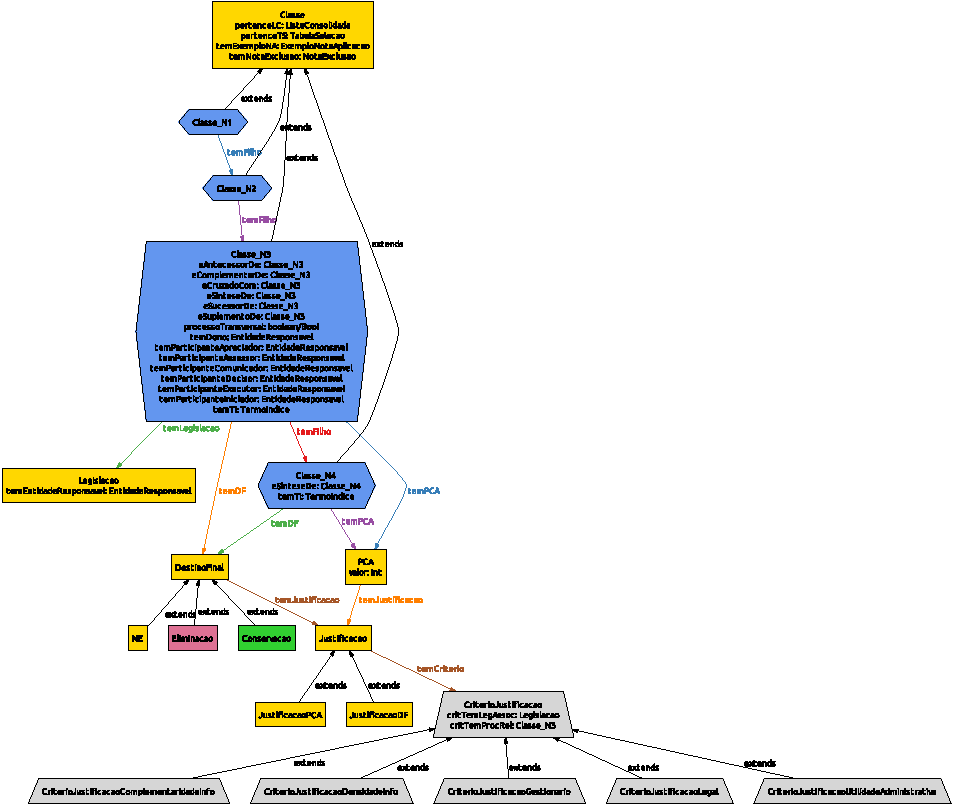
\includegraphics[width=\linewidth]{metamodel.pdf}
\caption{Meta-modelo simplificado}
\label{metamodel}
\end{figure}

Cada instituição pública portuguesa desempenha uma função específica dentro da AP (p. ex. a prestação de cuidados de saúde), associado a cada função existe um conjunto de várias sub-funções (p. ex. a gestão de utentes e serviços clínicos) e cada sub-função possui uma lista de processos de negócio que, concretamente, se materializam em documentos (p. ex. um processo de negócio pertencente à sub-função de gestão de utentes seria o registo clínico de utentes). A Lista Consolidada (LC) possui esta estrutura hierárquica de 4 níveis\cite{clav-mod} onde os processos de negócio são passíveis de ser desdobrados para efeitos de avaliação. Cada classe da LC possui um conjunto de atributos que a descreve e a partir do 3º nível (PNs) começam a surgir relações mais complicadas entre processos no campo chamado contexto de avaliação. Este contexto de avaliação, como também iremos ver mais à frente, tem associado um conjunto de invariantes que influenciarão o campo das decisões de avaliação. Este último campo é responsável por conter a informação sobre o Prazo de Conservação Administrativa (PCA) e Destino Final (DF) de um processo que correspondem, respetivamente, ao prazo que o documento deve ser guardado e qual o seu destino uma vez que este prazo expire.

Embora as entidades principais no domínio do problema sejam as classes da LC, existem várias outras que se relacionam direta ou indiretamente com cada uma das classes e que fornecem uma maior profundidade e complexidade ao modelo como podemos observar na figura \ref{metamodel}.

Observando o meta-modelo simplificado, onde a azul se encontram os 4 nivéis de classe, verificamos que este possui uma complexidade natural mesmo sem lhe impor alguma restrição. Sendo assim, e dado o contexto sério em que o problema está inserido, torna-se claro que deve ser feita alguma coisa no que diz respeito a dar algumas garantias acerca da coerência e consistência da LC.

\subsection{Primeiro \textit{Checkpoint}}

Sendo o CLAV um projeto que já existe há 1 ano e já se encontra com alguns componentes operacionais, decidiu-se pegar em toda a documentação existente sobre o modelo e os seus requisitos e, com a ajuda do Professor José Carlos Ramalho, fazer um apanhado de todas as entidades e relações existentes. Durante esta primeira fase, bastantes das reuniões semanais serviram para apurar pequenos detalhes e dúvidas que iam surgindo.

Uma das razões que motivaram este investimento inicial, apesar de já existir uma ontologia definida pela qual nos podíamos guiar, foi a de existir muita documentação\cite{clav-new}\cite{clav-mod}\cite{clav-req} solta e incompleta que nem sempre estava de acordo com a versão mais recente da ontologia. Foi então, elaborado um documento, atualizado, que documenta os mais recentes requisitos e invariantes e que já se tornou bastante útil no refinamento da ontologia original, nomeadamente na eliminação de entidades e relações obsoletas e no apuramento do domínio e contradomínio de várias relações.

Na Secção \ref{SecModel} iremos falar mais detalhadamente sobre cada entidade e relação do modelo e na secção \ref{SecAlloy} será abordada a respetiva implementação em Alloy.

\subsection{Segundo \textit{Checkpoint}} \label{Sec2CheckP}

Uma das principais motivações deste projeto é estudar a forma como os mais variados invariantes interagem entre si e se, de alguma forma, se contradizem. É neste sentido que o Alloy, sendo uma linguagem de modelação de software leve que nos permite especificar tanto o modelo como as restrições a ele associadas, ajuda a detetar erros ingénuos e subtis.

Após o investimento inicial em colecionar todo o material relevante e necessário sobre o problema, deu-se início ao ciclo de vida de verificação do problema \cite{jno}. Apesar dos invariantes serem abordados com mais detalhes na secção \ref{SubSecInv}, é possível adiantar já que foram identificadas 38 restrições no total, sendo que 23 dessas foram acrescentadas no tal processo de verificação.

Podemos então concluir, que o Alloy teve um impacto positivo na análise das restrições do modelo e na especificação do modelo formal. É importante realçar que a utilização de um \textit{model checker} não descarta a necessidade de prova mas é muito útil para encontrar falhas de \textit{design} como pudemos constatar. A ausência de contra-exemplos dá uma grande confiança de que uma prova de correção está ao alcance.

\subsection{Avaliação Final}

Depois de validado o modelo e os seus invariantes de forma estática, isto é,
apenas verificar que as restrições impostas são coerentes e que existem
instâncias capazes de habitar o modelo, o percurso natural no ciclo de vida de
verificação seria o de modelar a passagem do tempo e as suas ações possíveis
(p. ex. a inserção de novas classes). No entanto, devido a restrições de tempo,
seria mais produtivo ser capaz de observar que instâncias, presentes na base de
dados, é que não iam de encontro às várias restrições. Nesse sentido, em relação
à última fase do projeto foram traduzidos os invariantes em Alloy para
\textit{queries} SPARQL, motor de base de dados escolhido para armazenar toda a
informação.

Devido à dimensão do modelo e quantidade de invariantes, foi colocada a hipótese
de traduzir, automaticamente, as \textit{queries} dada uma especificação.

Sendo assim, a terceira e última fase do trabalho consistiu na tradução manual
dos invariantes Alloy mais específicos para \textit{queries} SPARQL e na
exploração e desenvolvimento de uma prova de conceito capaz de gerar
automaticamente  \textit{query}. Estes dois últimos pontos serão explicados com
maior detalhe na secção \ref{SecQueries}

\section{Modelo Formal} \label{SecModel}

Nesta secção será abordada a especificação formal do CLAV. Será introduzida alguma notação relativa ao cálculo relacional utilizado na formalização do problema e, posteriormente, tanto as classes presentes no domínio do modelo como as relações entre estas serão enunciadas. Por último, devido à grande quantidade de invariantes existentes, apenas serão apresentados 3, que melhor ilustram a dimensão e complexidade do CLAV. A formalização apresentada nesta secção, assim como a especificação dos invariantes em notação relacional teve o contributo e ajuda do professor José Nuno Oliveira.

\subsection{Calcular com relações\cite{jno}\cite{jno-5}}

Dentro do contexto do CLAV podemos encontrar frases do género \textit{"A gestão de utentes é uma subfunção da prestação de cuidados de saúde"}, \textit{"O processo de referenciação de utentes para consultas é cruzado com o processo de registo nacional de utentes"} ou \textit{"Se um processo é complementar de outro, então o seu destino final é de conservação"}. Estas expressões podem ser interpretadas como relações tipadas entre objetos.

As relações, como as frases a cima, já existem na matemática há vários anos e possuem uma notação própria capaz de as exprimir. Em geral, a notação (infixa) \textit{b R a}, onde \textit{a} e \textit{b} são os objetos e \textit{R} a relação, é a que expressa mais naturalmente as relações. Esta notação aplica-se também ao uso da voz passiva, que expressa a relação inversa de \textit{R}, denotada por \textit{Rº}, onde \textit{b R a} significa o mesmo que \textit{a Rº b}. Por exemplo, \textit{é síntese deº = é sintetizado por}.\label{rel_inv}

Também é importante observar que relações do género \textit{R = é o pai de}, são relações em que quando conhecido, o pai (p. ex. de uma classe) é único. Relações com esta propriedade são referidas como \textit{simples} e satisfazem a propriedade

\begin{equation}
\label{eq-simple}
R \circ Rº \subseteq id
\end{equation}

\noindent onde ($\circ$), denota a composição de relações, \textit{id} é a relação identidade e $\subseteq$ é a inclusão de relações:

\begin{equation}
\label{eq-subseteq}
R \subseteq S \equiv \forall b; a : b R a \Rightarrow b S a.
\end{equation}

\subsubsection{Relações tipadas e diagramas:}

O uso de setas e diagramas torna possível expressar formulas relacionais mais complexas. No entanto, para ser possível representar e raciocinar sobre estes diagramas é necessário que estes estejam bem construídos.

Observando a relação \eqref{eq-subseteq} concluímos que apenas faz sentido se \textit{R} e \textit{S} forem do mesmo tipo. A notação $B \xleftarrow[]{\text{R}} A$ declara uma relação binária que relaciona \textit{B's} com \textit{A's}. Por exemplo, B = \textit{Classe nível 1} e A = \textit{Classe nível 2} para o caso em que \textit{R = é o pai de}. 

Caminhos em diagramas são construídos a partir do encadeamento de setas, o que corresponde à composição de relações:

\begin{equation}
\label{eq-composition}
\begin{tikzcd}
A \arrow[bend right, leftarrow, swap]{rr}{R\ \circ\ S} \arrow[leftarrow]{r}{R} & B \arrow[leftarrow]{r}{S} & C
\end{tikzcd}
\hskip2cm b (R \circ S) c \equiv \exists a: b R a \land a S c
\end{equation}

Os diagramas também advêm da comparação de caminhos, por exemplo,

\begin{center}
\begin{tikzcd}[row sep=tiny]
Classe\_N2 \arrow[swap]{dd}{temFilho12} &           & ListaConsolidada \arrow[swap]{ll}{pertenceLC2} \arrow{dd}{id} \\
                                      & \subseteq &                                                       \\
Classe\_N1                      &           & ListaConsolidada \arrow{ll}{pertenceLC1}  
\end{tikzcd}
\end{center}

\noindent que representa a restrição

\begin{equation}
\label{eq-inv1}
    temFilho12 \circ pertenceLC2 \subseteq id \circ pertenceLC1,
\end{equation}

\noindent onde, no domínio do CLAV, as relações \textit{pertenceLC1} e \textit{pertenceLC2} mapeiam, respetivamente, cada classe de nível 1 na sua respetiva LC e cada classe de nível 2 na sua respetiva LC, a relação simples, \textit{temFilho12}, relaciona uma classe de nível 1 com os seus filhos (classes de nível 2), a relação \textit{id} é a conhecida relação identidade que relaciona cada objeto consigo próprio.

\subsubsection{Dos diagramas à lógica\cite{jno}\cite{jno-5}:}

O que é que a expressão \eqref{eq-inv1} significa em lógica proposicional?

\begin{equation*}
    temFilho12 \circ pertenceLC2 \subseteq id \circ pertenceLC1
\end{equation*}
$\equiv$ \{ inclusão de relações \eqref{eq-subseteq}; id \}
\begin{equation*}
    \forall\ c1, lc : c1\ (temFilho12 \circ pertenceLC2)\ lc \Rightarrow c1\ pertenceLC2\ lc
\end{equation*}
$\equiv$ \{ composição (3) \}
\begin{equation*}
    \forall\ c1, lc : (\exists\ c2 : c1\ temFilho12\ c2\ \land\ c2\ pertenceLC2\ lc) \Rightarrow c1\ pertenceLC1\ lc
\end{equation*}
$\equiv$ \{ \textit{splitting; nesting} \}
\begin{equation*}
    \forall\ c1, c2, lc : c2\ pertenceLC2\ lc \land c1\ temFilho12\ c2\ \Rightarrow \ c1\ pertenceLC1\ lc
\end{equation*}

\noindent Literalmente:
\vskip0.2cm
\textit{Se uma c2 pertence à lista consolidada lc e c2 é filho da classe c1, então c1 também pertence à lista consolidada lc.}

\vskip0.2cm
\noindent Ainda em menos palavras, a restrição \eqref{eq-inv1}, sugere:
\vskip0.2cm
\textit{Filho de quem pertence, também pertence.}

\subsection{Domínio}

%Introduzir cada uma das signatures e o seu contexto no problema.
Com a especificação do domínio do modelo formal pretendemos descrever a essência do problema em questão que é o de garantir que, dadas as entidades existentes e as suas relações, o conjunto de invariantes impostos são coerentes, não se contradizem e permitem instâncias semanticamente corretas.

Sendo assim, nesta secção e na próxima, apesar do domínio especificado ser maior, apenas iremos apresentar as especificações que melhor capturam a essência do modelo, por questões de síntese. No entanto, será possível consultar o modelo na totalidade em anexo.

\subsubsection{Referencial Classificativo:}

O Referencial Classificativo possui o conjunto de Listas Consolidadas e Tabelas de Seleção onde se encontram as diversas funções (classes de nível 1).

\begin{equation*}
    ReferencialClassificativo = ListaConsolidada + TabelaSelecao
\end{equation*}

\subsubsection{Classes:}

Como já foi referido existem 4 níveis de classes e, como veremos na secção abaixo dá-nos jeito especificá-las da seguinte maneira.

\begin{equation*}
    Classes = Classe\_N1 + Classe\_N2 + Classe\_N3 + Classe\_N4
\end{equation*}

\subsubsection{PCA:}

O Prazo de Conservação Administrativa é o simples tipo de dados:

\begin{equation*}
    PCA
\end{equation*}

\subsubsection{Destino Final:}

O Destino Final é passível de ser avaliado em um de três valores: \textit{Não Especificado (NE)}, \textit{Eliminação} (quando o processo de negócio tem o destino de ser eliminado) e \textit{Conservação} (quando o processo de negócio deve ser preservado). Apesar de apenas existirem estes 3 valores, foi necessário distingui-los em entidades individuais devido ao facto de cada instância de um DF estar relacionada com outras entidades. Sendo assim:

\begin{equation*}
    DestinoFinal = NE + Eliminacao + Conservacao
\end{equation*}

\subsection{Relações envolvidas}

Observando apenas as entidades definidas na secção anterior não é bem clara a existência de uma hierarquia nem é clara a existência do contexto de avaliação nas classes de nível 3. Isto deve-se ao facto de estas características apenas se evidenciarem ao analisar as relações envolvidas entre cada uma das entidades do domínio.

É de realçar que foi feito um esforço em manter as nomenclaturas da ontologia original e devido a isso, muitas das relações inversas possuem nomes diferentes. No entanto, para efeitos de simplificação e leitura utilizaremos a notação apresentada em \ref{rel_inv} e as restrições de domínio/contradomínio serão esclarecidas no nome das relações.

\subsubsection{Visão hierárquica:}

\begin{equation}
\label{vis_geral}
\begin{tikzcd}
ListaConsolidada \arrow{d}{pertenceLC1} \arrow[swap,bend right=67]{dd}{pertenceLC2} \arrow[swap,bend right=60]{ddd}{pertenceLC3} \arrow[swap,bend right=49]{dddd}{pertenceLC4} \\
Classe\_N1 \arrow{d}{temFilho12º}                                                                                                                                     \\
Classe\_N2 \arrow{d}{temFilho23º}                                                                                                                                     \\
Classe\_N3 \arrow{d}{temFilho34º}                                                                                                                                     \\
Classe\_N4                                                                                                                                                             
\end{tikzcd}
\end{equation}

A cima, nas relações da familia \textit{pertenceLC} o número associado a elas diz respeito ao nível da classe. Nas relações da família \textit{temFilho}\footnote{Na ontologia, a relação inversa é a \textit{temPai}}, o primeiro número diz respeito ao pai e o segundo ao filho. Sendo assim, com estas relações já é possível observar a cascata hierárquica das classes de processos da Administração Pública associadas a uma Lista Consolidada.

Com esta representação gráfica podemos também concluir que o sentido do invariante \ref{eq-inv1} também se aplica às relações apresentadas, dando origem a mais dois diagramas semelhantes mas para as classes filho.

\subsubsection{Processos de negócio:}

\begin{equation}
\label{vis_pn}
\begin{tikzcd}
            &  & Classe\_N3 \arrow[loop,swap]{u}{\textit{\shortstack{eAntecessorDe \\ eComplementarDe \\ eCruzadoCom \\ eSinsteseDe \\ eSucessorDe \\ eSuplementoDe}}}                       &  &                                       \\
PCA \arrow{rru}{temPCA3} \arrow[swap, bend right]{rrrr}{temPCA4} &  & DestinoFinal \arrow[swap]{u}{temDF3} \arrow{rr}{temDF4} &  & Classe\_N4 \arrow[swap]{llu}{temFilho34}
\end{tikzcd}
\end{equation}

As endo-relações que dizem respeito aos processos de negócio na figura a cima são as principais relações presentes no contexto de avaliação e que irão influenciar o resultado do Destino Final. As classes de nível 4 são casos particulares em que um PN se desdobra com um certo motivo. Nesses casos as decisões de avaliação passam para os filhos. Como podemos ver, é nos processos de negócio que se encontra uma maior densidade de relações e é também nestes que se encontra a parte mais complexa e crítica do problema e, devido a isto, a maior parte dos invariantes irá focar-se neste diagrama. É de salientar que esta figura omite entidades e relações também relevantes que lidam com legislação e critérios de justificação que poderão ser encontrados no modelo final em anexo.

\subsection{Invariantes} \label{SubSecInv}

Como já foi dado a perceber, neste projeto, apenas foi focado o domínio de relações entre cada entidade pertencente à Lista Consolidada e, dentro deste domínio reduzido, apenas foi explorado com mais profundidade a parte de classificação e avaliação de processos de negócio ignorando assim, muitas das relações de atributos e invariantes associados a estas. Como foi referido em \ref{Sec2CheckP}, foram especificados, no total, 38 invariantes sendo que, 23 desses foram adicionados como resultado deste projeto.

Tentando perceber o motivo por de trás de terem sido acrescentados tantos invariantes chegamos à conclusão de que, a maior parte deles incide em invariantes que dizem respeito à taxonomia das relações, onde a injetividade é a mais comum, e os restantes provêm do trabalho realizado neste projeto onde, em conjunto com o Professor José C. Ramalho, foram discutidos e validados e dizem respeito à parte semântica/funcional do CLAV.

\subsubsection{Injetividade:}

A injetividade garante que não existem duas instâncias da mesma entidade a relacionarem-se com uma outra entidade. Este invariante está presente em quase todas as relações uma vez que cada instância, principalmente ao nível dos PNs, está relacionada com legislação e critérios de justificação específicos e não faz sentido serem partilhados.

Generalizadamente, uma relação é injetiva quando:

\begin{equation}
\label{injetivity}
    ker\ R \subseteq id
\end{equation}

Concretamente e intuitivamente, à luz de \ref{vis_geral} e \ref{vis_pn}, uma classe não pode ter 2 pais diferentes (\ref{inv-inj-filho}) nem dois PNs (incluindo classes de nível 4) podem ter a mesma instância de DF (\ref{inv-inj-df}):

\begin{equation}
    \label{inv-inj-filho}
    ker\ temFilhoº \subseteq id
\end{equation}
\begin{equation}
    \label{inv-inj-df}
    ker\ temDF \subseteq id
\end{equation}

As restrições mais complexas envolvem são as que envolvem as endo-relações dos PNs e as que envolvem desdobramento ao 4º nível. Contextualizando, apesar de não ser frequente, um processo de negócio (nível 3) é passível de ser desdobrado em dois ou mais processos filho (nível 4) sendo que, podem existir dois motivos de desdobramento: DF distinto ou PCA distinto. As classes filho resultantes de tais desdobramentos possuem critérios de avaliação e classificação específicos que devem ser respeitados. Em baixo seguem-se 3 invariantes que caracterizam algumas das restrições impostas:

\begin{enumerate}
    \item Se uma classe de nível 3 tem filhos, então não possui DF nem PCA (o oposto caso não tenha filhos):
    
    \begin{equation}
    \label{inv-3-4}
    \begin{tikzcd}
                                                                                                                                                                                           &  &            & DF \arrow[swap]{ld}{temDF}                                       \\
Classe\_N4 \arrow{rr}{temFilho34} \arrow[bend left]{rrru}{temFilho34\backslash \neg temDF} \arrow[swap, bend right]{rrrd}{temFilho34\backslash \neg temPCA} \arrow[swap, bend right]{rrr}{R} &  & Classe\_N3 & DF \times PCA \arrow[swap]{u}{\pi_1} \arrow{d}{\pi_2} \\
                                                                                                                                                                                           &  &            & PCA \arrow{lu}{temPCA}                                     
\end{tikzcd}
    \end{equation}{}
    \begin{equation*}
        R = \langle (temFilho34\backslash \neg temDF), (temFilho34\backslash \neg temPCA) \rangle
    \end{equation*}{}
    
    \item Um PN só pode ter uma (endo) relação com outro PN:
    
    \begin{equation}
    \begin{split}{}
        eAntecessorDe \subseteq\ & \neg (eComplementarDe \cap eCruzadoCom \\
                                & \cap eSinteseDe \cap eSintetizadoPor \\
                                & \cap eSucessorDe \cap eSuplementoDe \\
                                & \cap eSuplementoPara)
    \end{split}{}
    \end{equation}{}
    
    A disjunção desta restrição com mais 7 do género (permutações entre o lado esquerdo e direito) formam a especificação da restrição completa.
    
    \item Se um PN é complementar ou sintese de outro, então o seu DF é de conservação; se é sintetizado por outro, então o seu DF é de eliminação; caso não seja nenhum dos especificados, o seu DF é NE (não especificado).
    
    Dividindo em várias cláusulas obtemos e assumindo que o PN não tem filhos:
    
    \begin{equation}
        eComplementarDe \backslash (temDF \circ \underline{Conservacao})
    \end{equation}{}
    \begin{equation}
        (\neg eComplementarDe \cap eSinteseDe) \backslash (temDF \circ \underline{Conservacao})
    \end{equation}{}
    \begin{equation}
    \begin{split}
        & (\neg eComplementarDe \cap \neg eSinteseDe \cap eSintetizadoPor) \\
        & \backslash (temDF \circ \underline{Eliminacao})
    \end{split}{}
    \end{equation}{}
    \begin{equation}
    \begin{split}
        & (\neg eComplementarDe \cap \neg eSinteseDe \cap \neg eSintetizadoPor) \\
        & \backslash (temDF \circ \underline{NE})
    \end{split}{}
    \end{equation}{}
\end{enumerate}
% Falar/Enumerar/Explicar alguns invariantes

\section{Modelação em ALLOY} \label{SecAlloy}

A partir do momento em que a formalização está completa resta-nos verificar se, dados os invariantes e a sua conjunção, existem instâncias capazes de habitarem o modelo. Uma solução seria, aleatoriamente e manualmente, popular os conjuntos de cada entidade e de forma \textit{ad hoc} e dispendiosa, verificar se aquele conjunto poderia habitar o modelo. Outra solução bastante mais eficaz será a de recorrer a um \textit{model checker} que, de forma automática, faz essa geração e verificação por nós. As ferramentas de \textit{model checking} tornam o ciclo de vida de verificação muito mais produtivo.

É aqui que o Alloy Analyzer tem impacto e ajuda a perceber que tipo de refinamento deve ser dado ao modelo formalizado e de que maneira é que os invariantes têm impacto nas instâncias possíveis. Nesta secção será abordada a maneira como foi feita a tradução do modelo formal, assim como os seus invariantes para Alloy.

\subsection{Especificação}

Começando pelo domínio do modelo, a cada entidade corresponderá uma \textit{sig} em Alloy. A noção de herança, capturada pelas Classes, Referencial Classificativo e Destino Final é traduzida pelas primitivas \textit{abstract} e \textit{extends}, inspiradas pela programação orientada a objetos. Sendo Assim:

\begin{verbatim}
abstract sig ReferencialClassificativo {}
sig ListaConsolidada extends ReferencialClassificativo {}
sig TabelaSelecao extends ReferencialClassificativo {}

/* ---- */

abstract sig Classe {}

sig Classe_N1 extends Classe {}
sig Classe_N2 extends Classe {}
sig Classe_N3 extends Classe {}
sig Classe_N4 extends Classe {}


/* ---- */

abstract sig DestinoFinal {
    temJustificacao: one Justificacao
}
sig Eliminacao, Conservacao, NE extends DestinoFinal {}
\end{verbatim}{}

No que diz respeito às relações envolvidas, o Alloy permite especificar as relações entre cada entidade da seguinte forma:

\begin{verbatim}
sig Classe_N1 extends Classe {
    temFilho: set Classe_N2,
}
\end{verbatim}{}

Como podemos ver, está definida uma relação $Classe\_N2 \xleftarrow[]{\text{temFilho}} Classe\_N1$ com uma cardinalidade \textit{set} no contradomínio, ou seja, $temFilho$ é uma relação de 0 para muitos. Mais concretamente, a relação especificada é a relação $temFilho12$ como podemos concluir olhando para o domínio e contradomínio. Uma última nota em relação à forma como foi traduzido o modelo, é a de que apesar de ser mais intuitivo na notação relacional representar uma relação como $y R x$, onde $Y \xleftarrow[]{\text{R}} X$, em Alloy é mais intuitivo modelar da forma $x R y$. Mesmo a composição relacional é feita da esquerda para a direita, ao contrário da notação relacional.

\subsection{Verificação}

O Alloy permite especificar expressões em lógica de primeira ordem. Para isso, disponibiliza as palavras reservadas \textit{all} e \textit{some} para quantificar universalmente e existencialmente, respetivamente, variáveis tipadas no universo modelado.

Uma das vantagens de utilizar a ferramenta Alloy é a de tudo poder ser visto como uma relação o que ajuda na tradução do modelo em si, como vimos na secção anterior, mas também permite fazer uma tradução praticamente direta dos invariantes em notação relacional \textit{point wise}, com o auxilio dos quantificadores, ou \textit{point free}, com o auxilio da composição de relações.

Com isto, e pela mesma ordem, segue-se a tradução dos invariantes apresentados em \ref{SubSecInv}:
\begin{enumerate}
    \item
    \label{inv-simples}
    \begin{verbatim}
all c:Classe_N3 | 
    some c.temFilho => no c.temDF and no c.temPCA
    \end{verbatim}{}
    
    \item
    \begin{verbatim}
all c1,c2:Classe_N3 | 
    c1->c2 in eAntecessorDe 
        => c1->c2 not in eComplementarDe + eCruzadoCom 
                         + eSinteseDe + eSintetizadoPor 
                         + eSucessorDe + eSuplementoDe 
                         + eSuplementoPara
    \end{verbatim}{}
    
    \item
    \begin{verbatim}
all c:Classe_N3 | no c.temFilho => {
    some c.eComplementarDe => c.temDF in Conservacao
}
all c:Classe_N3 | no c.temFilho => {
    !(some c.eComplementarDe) and (some c.eSinteseDe) 
        => c.temDF in Conservacao
}
all c:Classe_N3 | no c.temFilho => {
    !(some c.eComplementarDe) and !(some c.eSinteseDe) 
    and (some c.eSintetizadoPor) 
        => c.temDF in Eliminacao
}
all c:Classe_N3 | no c.temFilho => {
    !(some c.eComplementarDe) and !(some c.eSinteseDe) 
    and !(some c.eSintetizadoPor) 
        => c.temDF in NE
}
    \end{verbatim}{}
\end{enumerate}{}

\section{Tradução de \textit{queries} SPARQL}
\label{SecQueries}

Um modelo formal em Alloy permite raciocinar, utilizando cálculo relacionar e
métodos matemáticos, sobre o problema e, tirando partido do \textit{model
checker} eliminar erros de conceção ingénuos ou que possam ter passado
despercebidos. O modelo apresentado nas secções anteriores é apenas um modelo
estático sendo que sabemos apenas, com alguma certeza, de que este é passível de
ser habitado. No entanto, são necessárias operações sobre este para que evolua,
a partir de um estado inicial. Entre outras, estas operações correspondem a
ações de inserção, atualização, remoção de instâncias no modelo e não devem
permitir que as restrições impostas sejam violadas.

Um próximo passo na especificação do modelo formal do CLAV seria o de
especificar tais ações estudando assim a passagem do tempo e que tipo de
propriedades, tanto de \textit{safety} como de \textit{liveness}, seriam
verificadas. Mas, devido ao estado avaçado do projeto, um passo alternativo no
contexto do CLAV, mais produtivo uma vez que já se encontra em produção, é o de
a partir da especificação dos invariantes, traduzi-los em \textit{queries}
SPARQL que apanhem as instâncias da base de dados que não verificam as
restrições impostas. Desta forma, será fácil identificar as anomalias no sistema
e resolvê-las.

A tradução dos invariantes poderá ser feita de duas formas: manualmente ou
automaticamente. Nas secções abaixo será explicada de que forma é que ambas
estas formas de tradução podem ser executadas.

\subsection{Tradução manual}

Numa primeira vista, a sintaxe de uma \textit{query} SPARQL, sendo este motor
orientado a grafos, é bastante semelhante à de um motor de bases de dados
relacional como podemos ver em baixo.

\begin{verbatim}
PREFIX P: <URI>

SELECT ?Property1 ?Property2

WHERE {
    ?v1 P:rel1 ?Property1 .
    ?v1 P:rel2 ?Property2 .
}
\end{verbatim}

Resumidamente e como podemos observar, o processador SPARQL funciona com
\textit{pattern matching} de triplos RDF. Baseado em lógica de primeira ordem e
teoria de conjuntos, suporta operadores como a união e interseção de resultados,
que permitem uma manipulação dos resultados de forma bastante simples e
intuitiva.

A partir desta informação e sabendo que o Alloy é baseado em lógica de primeira
ordem e álgebra relacional, é possível inferir que estas duas linguagens possuam
bastantes semelhanças. A verdade é que para os invariantes mais simples a
tradução é quase direta havendo apenas o pequeno pormenor de que é necessário
especificar a \textit{query} na forma do invariante negado e em formato CNF
(\textit{Conjunctional Normal Form}).

Ilustrando então com um exemplo simples, como o invariante \ref{inv-simples}, a
sua forma negada será:

\begin{verbatim}
some c:Classe_N3 | 
    (some c.temFilho) and ((some c.temDF) or (some c.temPCA))
\end{verbatim} 

A tradução manual deste invariante passa por analisar o tipo de variavéis a
identificar onde, neste caso, serão do tipo \texttt{Classe\_N3} e filtrar os
resultados pelas instâncias que verificam as condições impostas no corpo do
invariante. O processador SPARQL possui o operador FILTER que permite fazer esta
filtragem, resultando na queries seguinte:

\begin{verbatim}
PREFIX : <http://jcr.di.uminho.pt/m51-clav#>
PREFIX clav: <http://jcr.di.uminho.pt/m51-clav#>
PREFIX rdf: <http://www.w3.org/1999/02/22-rdf-syntax-ns#>
select * where {
   ?c rdf:type :Classe_N3 .
   ?c :temFilho ?cf .

    FILTER (
        EXISTS { ?c :temDF ?df . } ||
        EXISTS { ?c :temPCA ?pca . }
    )
}
\end{verbatim} 

\textit{Queries} mais complexas e que envolvam composição de funções, uma vez
que o SPARQL não é capaz de tal funcionalidade, a \textit{query} deve
explicitamente unificar as variáveis de forma obter o mesmo comportamento.
Veja-se o exemplo:

\begin{verbatim}
some c:Classe_N3,t:c.temTI | 
    (some c.temFilho) and (t not in c.temFilho.temTI)
\end{verbatim} 

\begin{verbatim}
PREFIX : <http://jcr.di.uminho.pt/m51-clav#>
PREFIX clav: <http://jcr.di.uminho.pt/m51-clav#>
PREFIX rdf: <http://www.w3.org/1999/02/22-rdf-syntax-ns#>
select * where { 
    ?c rdf:type :Classe_N3 .
    ?c :temFilho ?cf .
    ?c :temTI ?ti .
   	
    FILTER (
        NOT EXISTS { ?cf :temTI ?ti . }
	)
}
\end{verbatim} 

Esta sistematização dá uma boa confiança de que a automação deste processo está
ao alcance.

\subsection{Geração automática}

Como vimos anteriormente, o processo de tradução da especificação de um
invariante em Alloy para um \textit{query} SPARQL passa por várias fases. A
primeira fase é a da negação do invariante em si, utilizando regras de lógica de
primeira ordem conhecidas. A segunda fase, passa por identificar as variáveis
quantificadas e o seu tipo sendo que, estas serão traduzidas em unificações do
tipo: \texttt{?var rdf:type :<Tipo>}. A terceira fase passa por identificar, no
corpo do invariante quais as condições que as variáveis unificadas devem
respeitar de forma a encontrar as instâncias incorretas da base de dados. Esta
última fase, tira partido do operador FILTER como mencionado na secção anterior.

Para ser possível sistematizar este processo é necessário carregar o invariante
numa estrutura que permita a sua manipulação de forma prática, ou seja, é
necessário efetuar o \textit{parsing} do invariante para uma estrutura de dados.
Para este efeito, recorreu-se ao par Happy + Alex, bibliotecas em Haskell que
permitem a especificação de uma gramática e de um \textit{lexer} e respetivas
ações semânticas apartir de uma DSL (\textit{Domain Specific Language}) bastante
semelhante à das ferramentas Yacc/Flex da linguagem C, para obter a árvore de
sintaxe, e à biblioteca \textit{recursion-schemes} para a sua manipulação. É de
salientar que o gerador desenvolvido tem como objetivo ser apenas uma prova de
conceito logo, é apenas capaz de efetuar o \textit{parsing} de um sub conjunto
bastante limitado da sintaxe Alloy e de gerar \textit{queries} a partir de
especificações bastante simples.

Tendo o \textit{parsing} feito, apenas é necessário transformar a estrutura
obtida fazendo-a passar pelas várias fases enunciadas em cima. A codificação das
várias fases em Haskell foi bastante simples devido à escolha de manter o nome
das relações usadas na ontologia base no modelo Alloy pois, não foi necessário
fazer nenhuma correspondência entre os nomes. Sendo assim, segue-se abaixo, a
\textit{query} gerada automaticamente a partir do invariante escolhido na secção
anterior:

\begin{verbatim}
PREFIX : <http://jcr.di.uminho.pt/m51-clav#> 
PREFIX clav: <http://jcr.di.uminho.pt/m51-clav#> 
PREFIX rdf: <http://www.w3.org/1999/02/22-rdf-syntax-ns#> 

SELECT * WHERE {


	 ?c rdf:type :Classe_N3 . 

	FILTER ( 
		EXISTS { 	
		 ?c :temFilho ?blG . 
		} 

	 && (
		EXISTS { 	
		 ?c :temDF ?76V . 
		} 

	 || 
		EXISTS { 	
		 ?c :temPCA ?FIn . 
		} 
        ))

}
\end{verbatim}

As \textit{queries} geradas são traduções corretas uma vez que ambas as
ferramentas (SPARQL e Alloy) são baseadas nos mesmo princípios teóricos logo,
partilham, à partida, de uma representação base (isomorfismo).

\section{Dificuldades}

%Documentação do projeto do CLAV:
%    - espalhada
%    - desorganizada
%    - desatualizada
%    Implicações:
%        - Tivemos que fazer o apanhado de tudo

%Alguns dos invariantes não eram estáveis e sofreram alterações ao longo do projeto assim como alguns pormenores relacionados com o modelo em si.

\section{Conclusão e Trabalho Futuro} \label{SecConclusion}

%
% ---- Bibliography ----
%
% BibTeX users should specify bibliography style 'splncs04'.
% References will then be sorted and formatted in the correct style.
%
% \bibliographystyle{splncs04}
% \bibliography{mybibliography}
%
\bibliographystyle{splncs04}
\bibliography{mybib}{}

\end{document}
